\chapter{Results}

% pre-figure explanation
  We rendered the resulting behaviors produced by controllers trained on aforementioned reward functions and environments into images or frames.
  Combining the frames generated for each of the 1000 timesteps and setting as 60 frames per second resulted in 33.35 second videos.
  The time-lapses presented in \ref{fig:manual_trajectory_body_speed_0}, \ref{fig:manual_trajectory_strict_body_speed_1}, \ref{fig:manual_trajectory_not_strict_body_speed_1}, \ref{fig:fifty_fifty_body_speed_0}, and \ref{fig:fifty_fifty_body_speed_1} were created by sampling every $300$ frames within the last 30 seconds of the video.
  The frames' sequential order is from the top left to the bottom right.
  The camera is locked to follow the pigeon's body.
  % 60/5 * [10] = 300


  \begin{figure}[H]
      \centering
      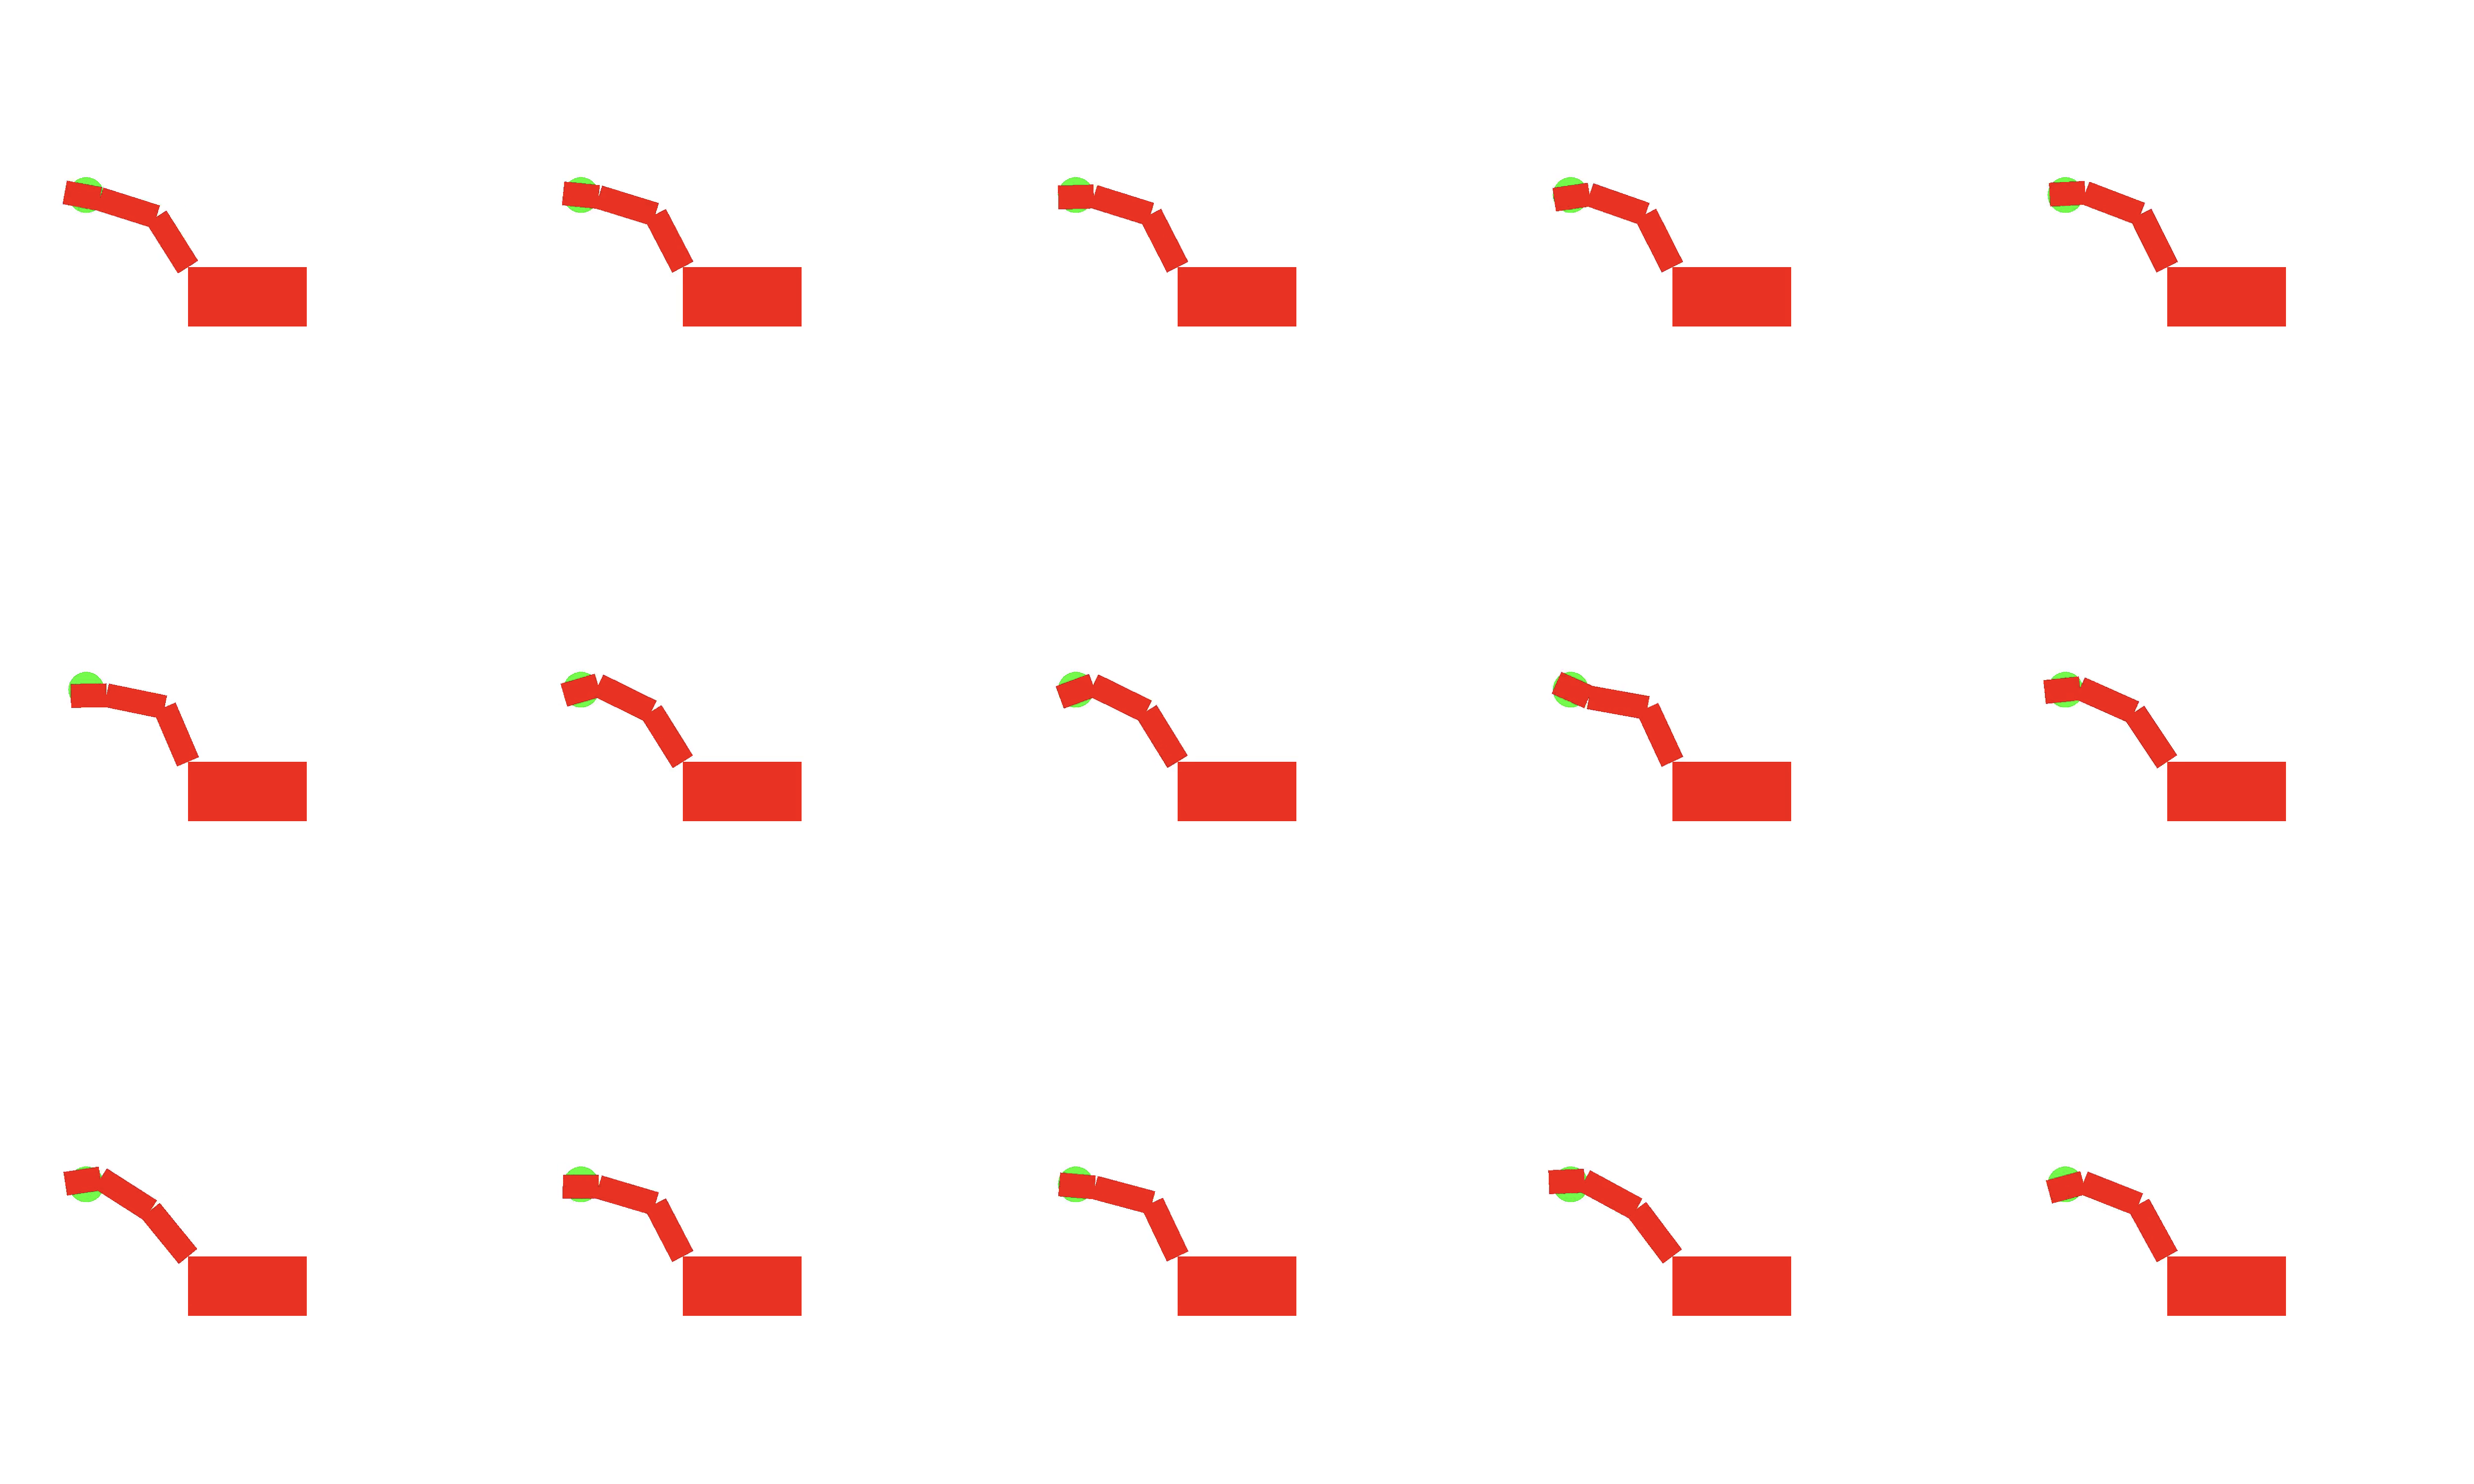
\includegraphics[width=1\textwidth]{figures/frames/frames_001.png}
      \caption{Control of a pigeon model with a static body trained on $r_{head\_stable\_manual\_reposition\_strict\_angle}$ with $max\_offset = 0.5$}
      \label{fig:manual_trajectory_body_speed_0}
  \end{figure}

  \begin{figure}[H]
      \centering
      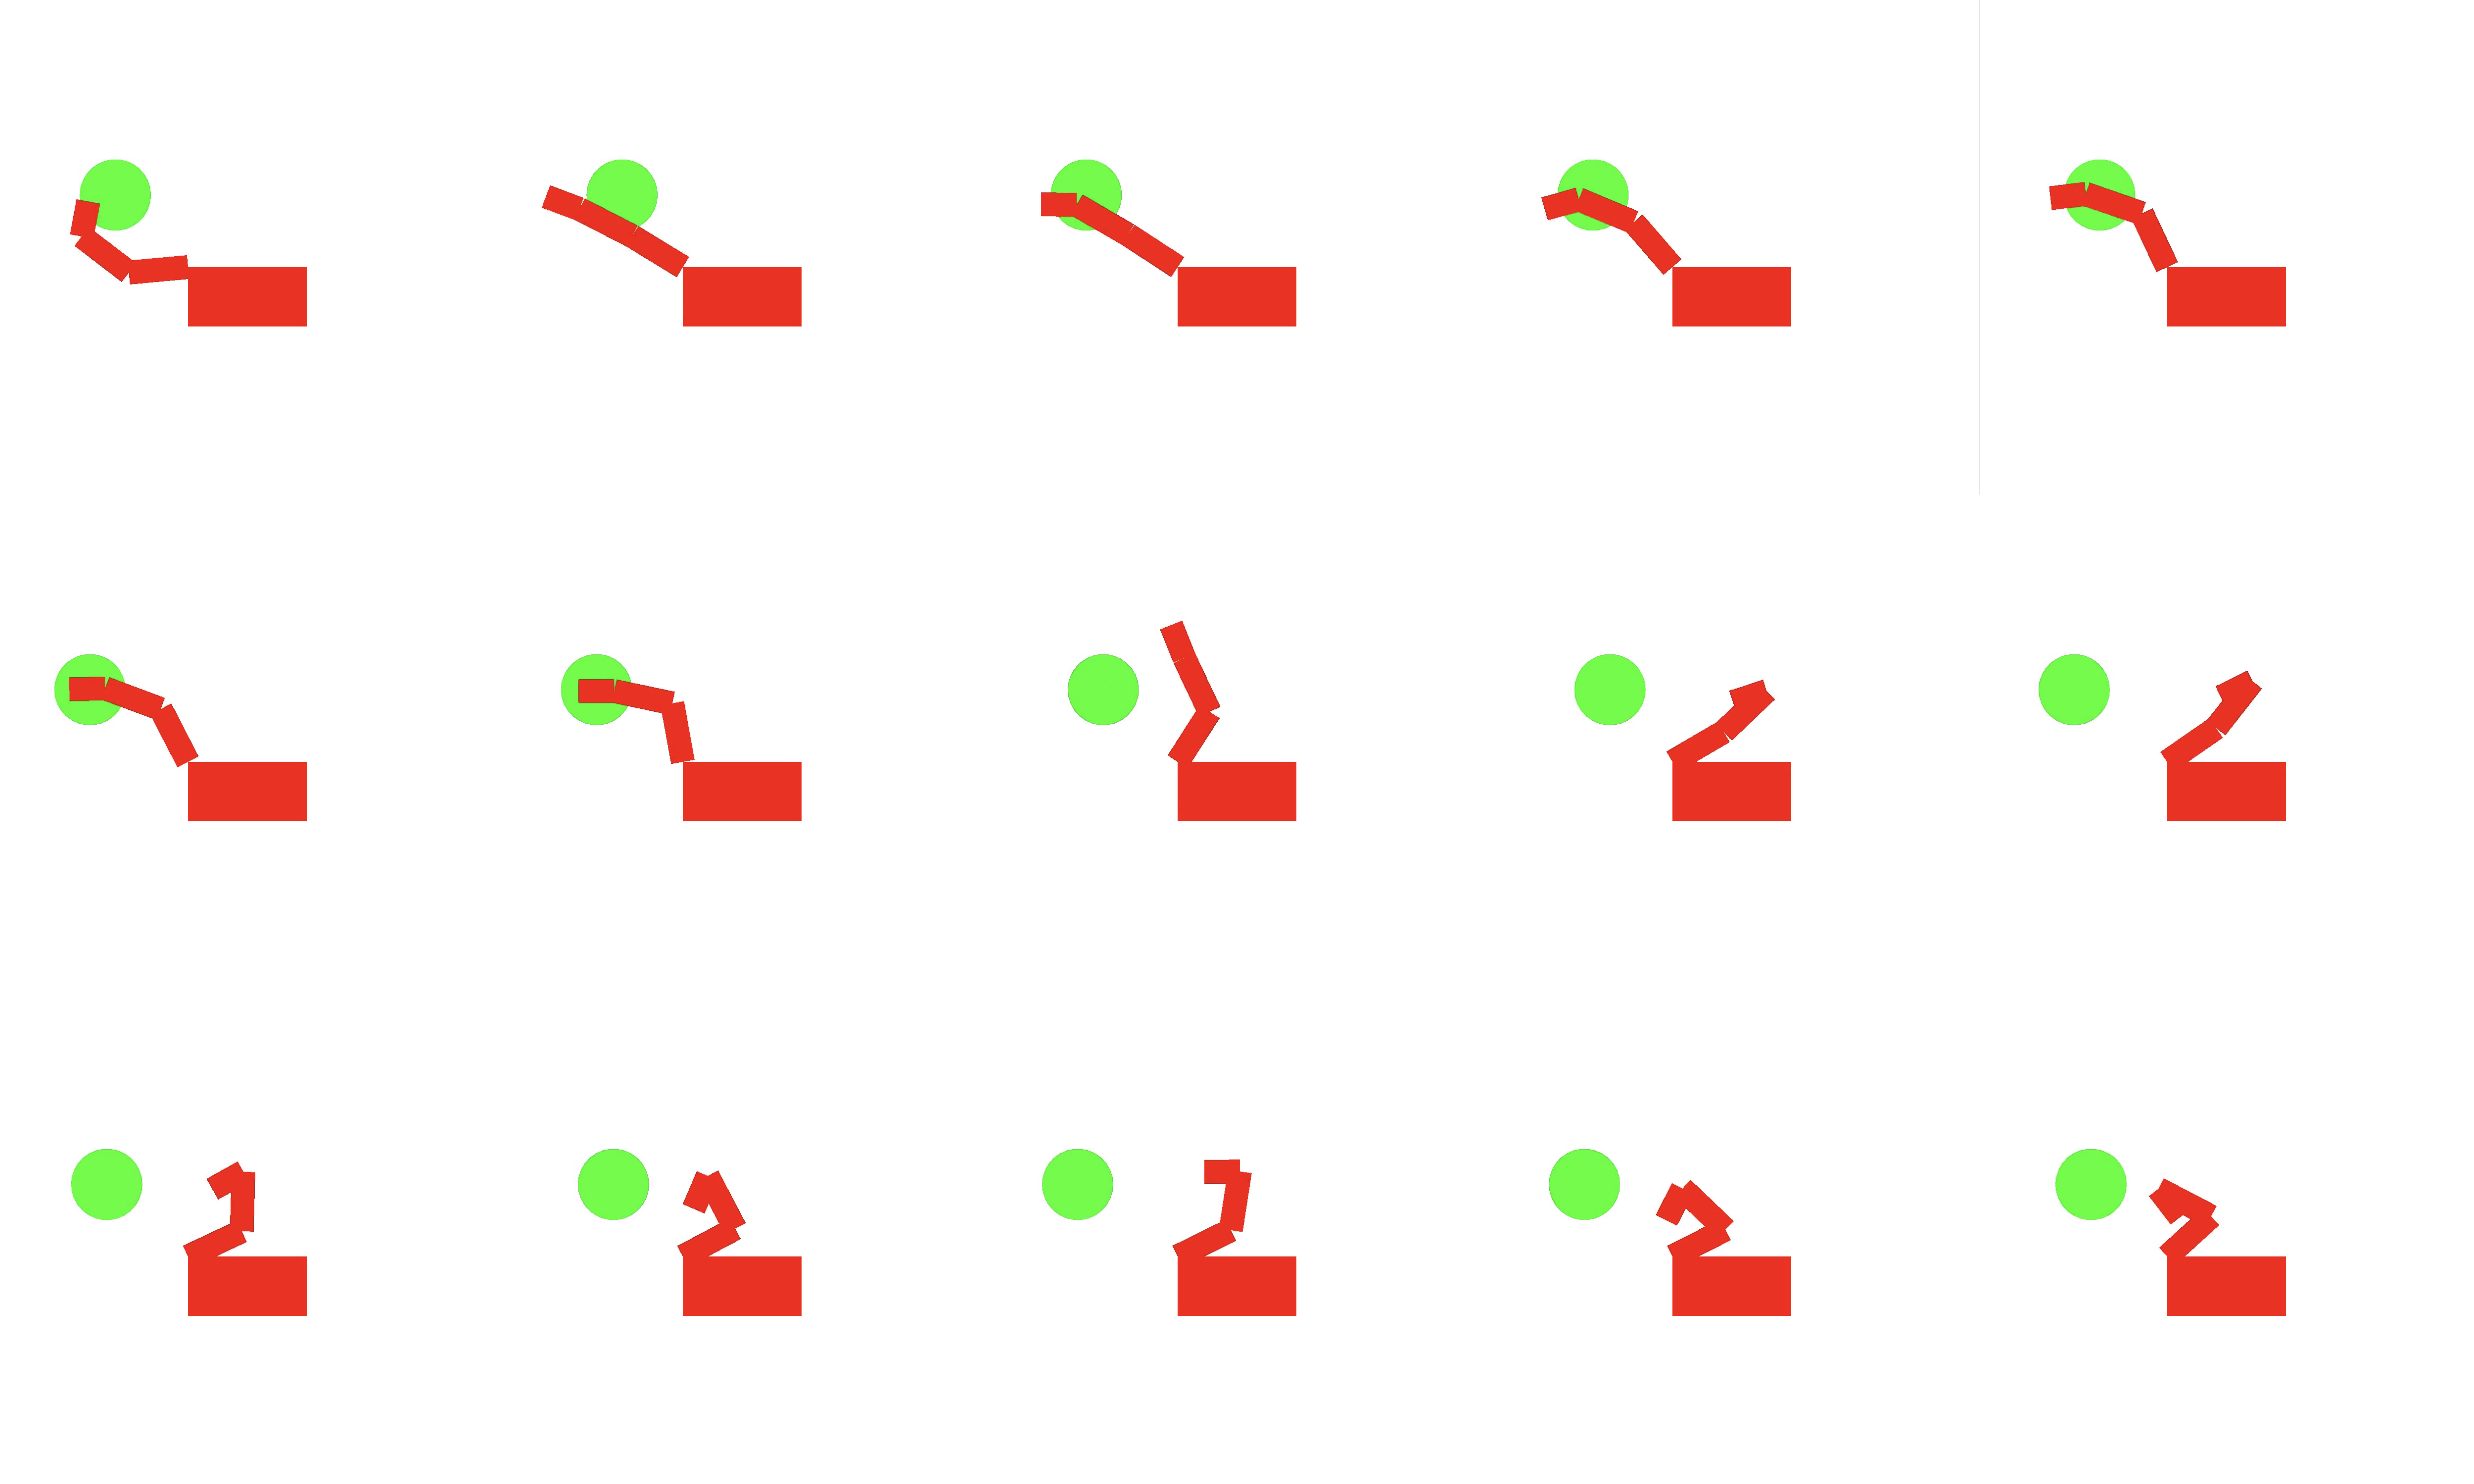
\includegraphics[width=1\textwidth]{figures/frames/frames_002.png}
      \caption{Control of a pigeon model with the body speed of 1 trained on $r_{head\_stable\_manual\_reposition\_strict\_angle}$ with $max\_offset = 1.0$}
      \label{fig:manual_trajectory_strict_body_speed_1}
  \end{figure}

  \begin{figure}[H]
      \centering
      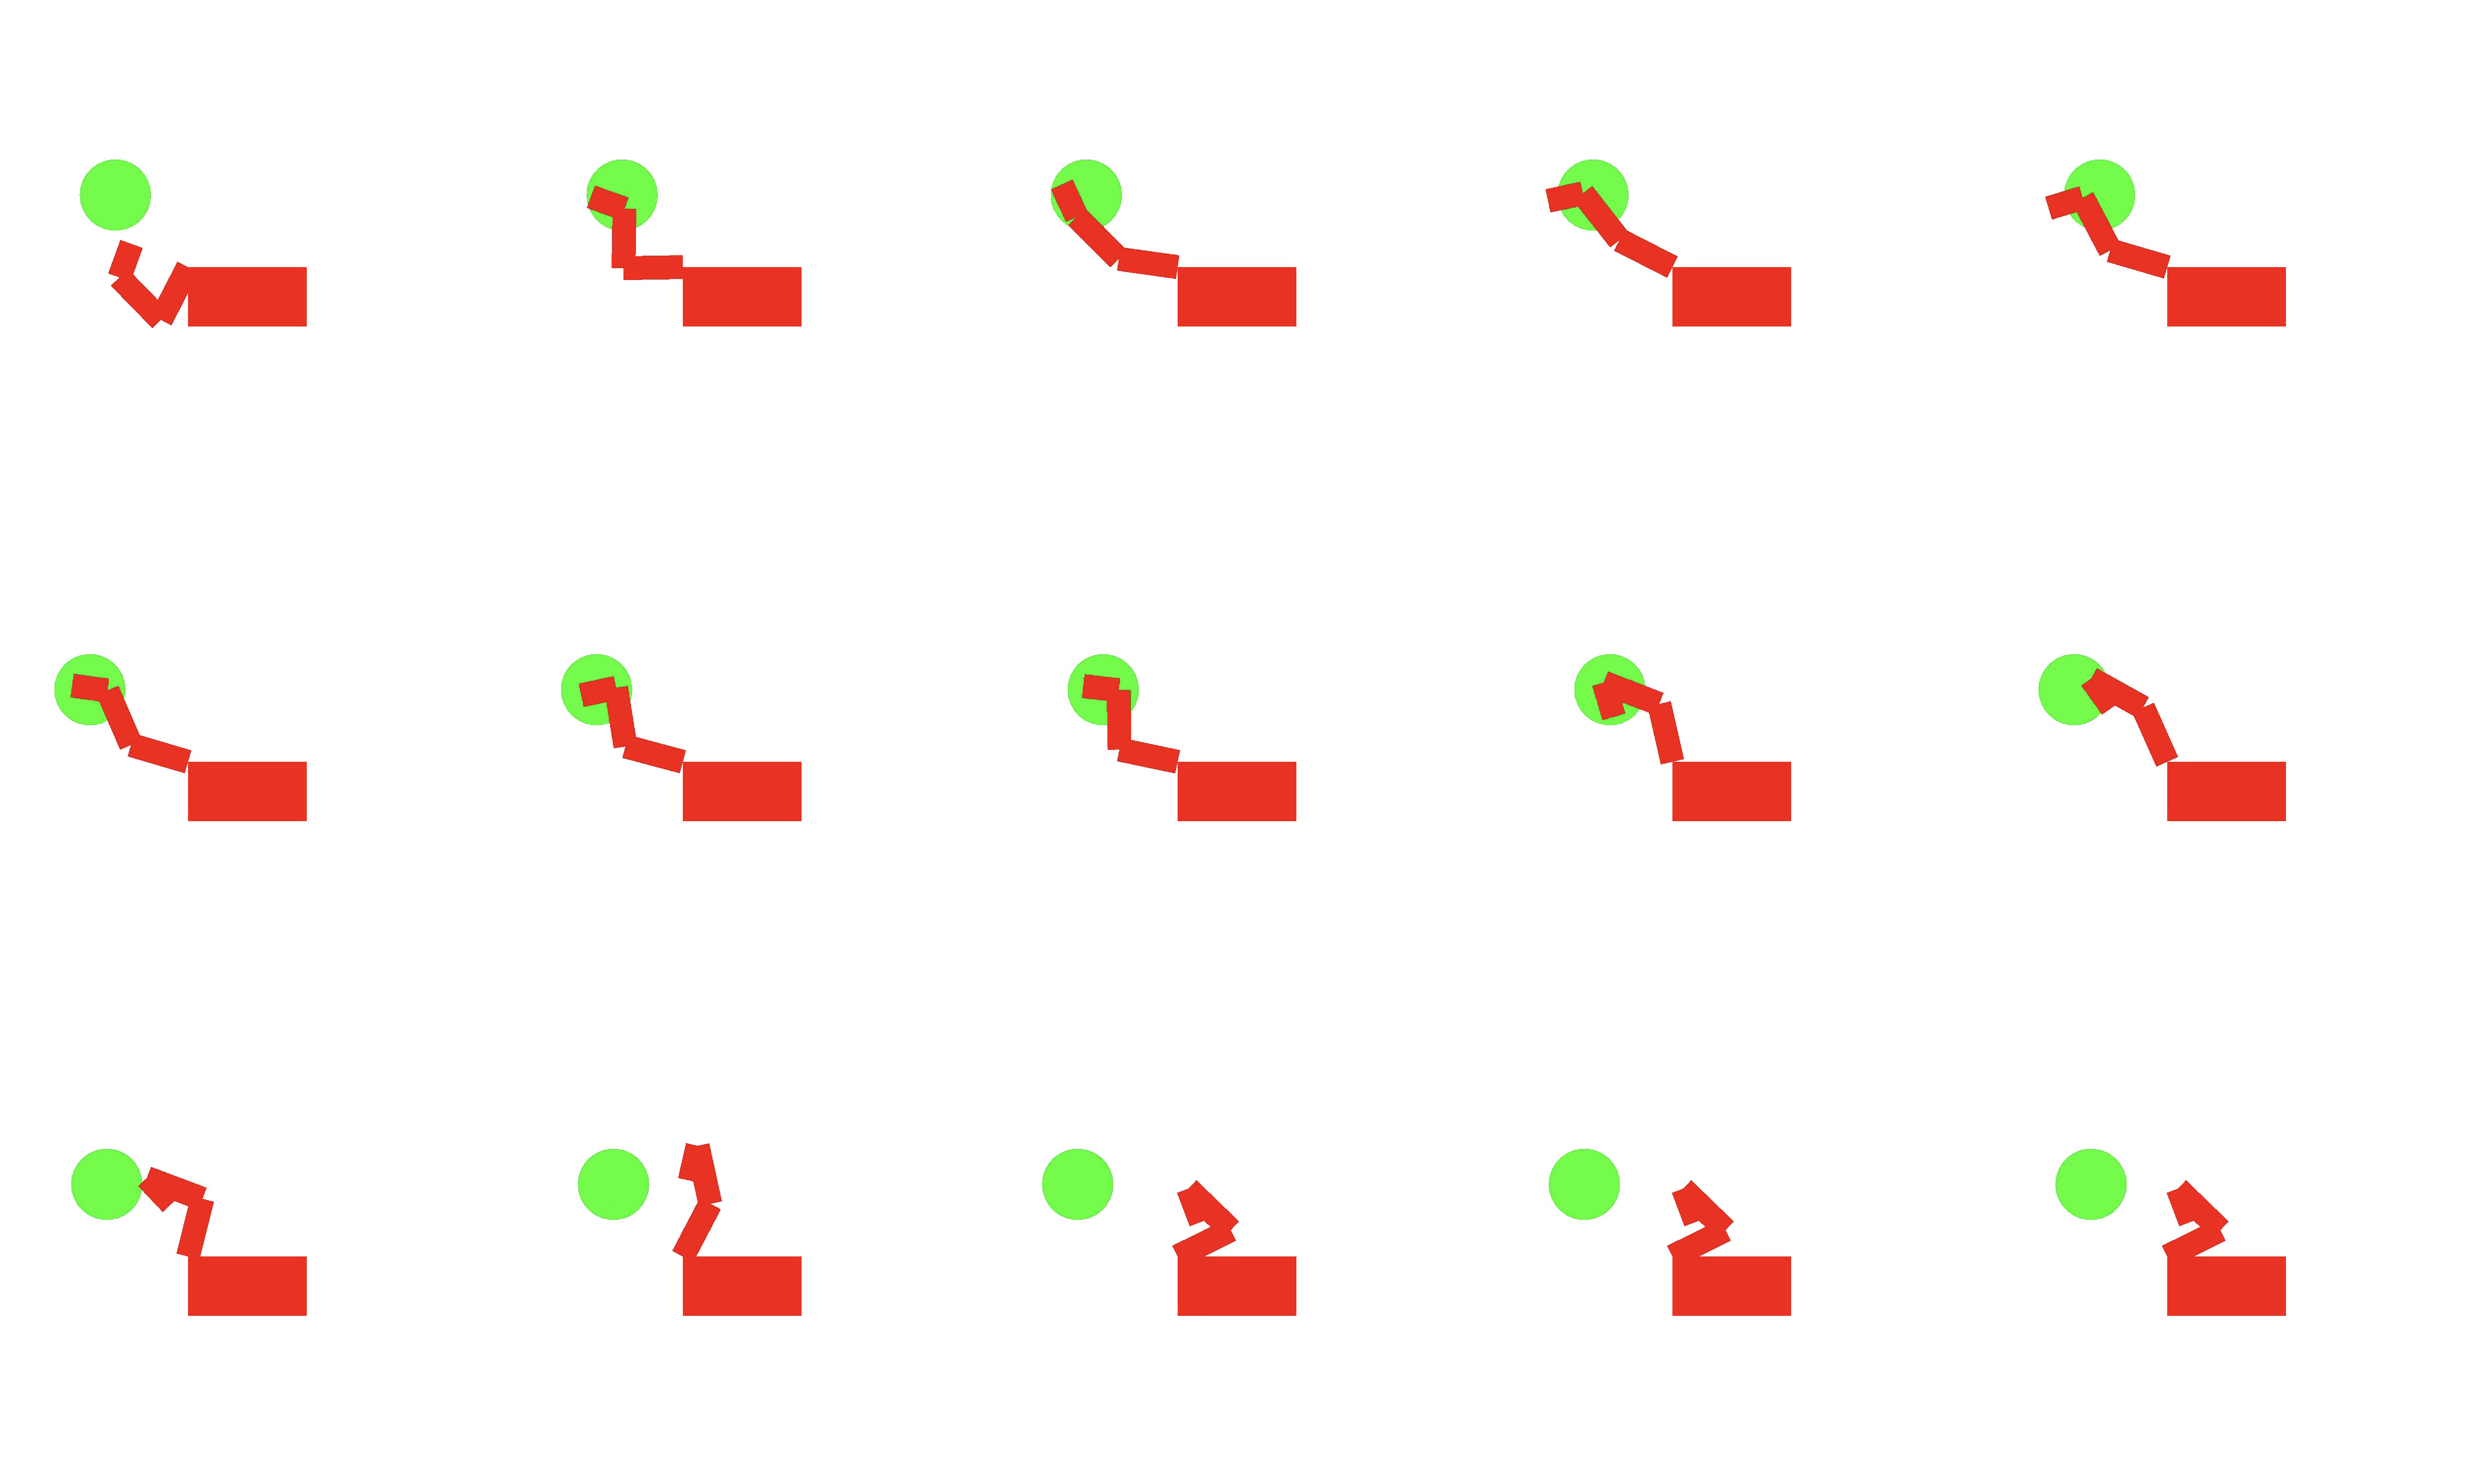
\includegraphics[width=1\textwidth]{figures/frames/frames_003.png}
      \caption{Control of a pigeon model with the body speed of 1 trained on $r_{head\_stable\_manual\_reposition}$ with $max\_offset = 1.0$}
      \label{fig:manual_trajectory_not_strict_body_speed_1}
  \end{figure}

  \begin{figure}[H]
      \centering
      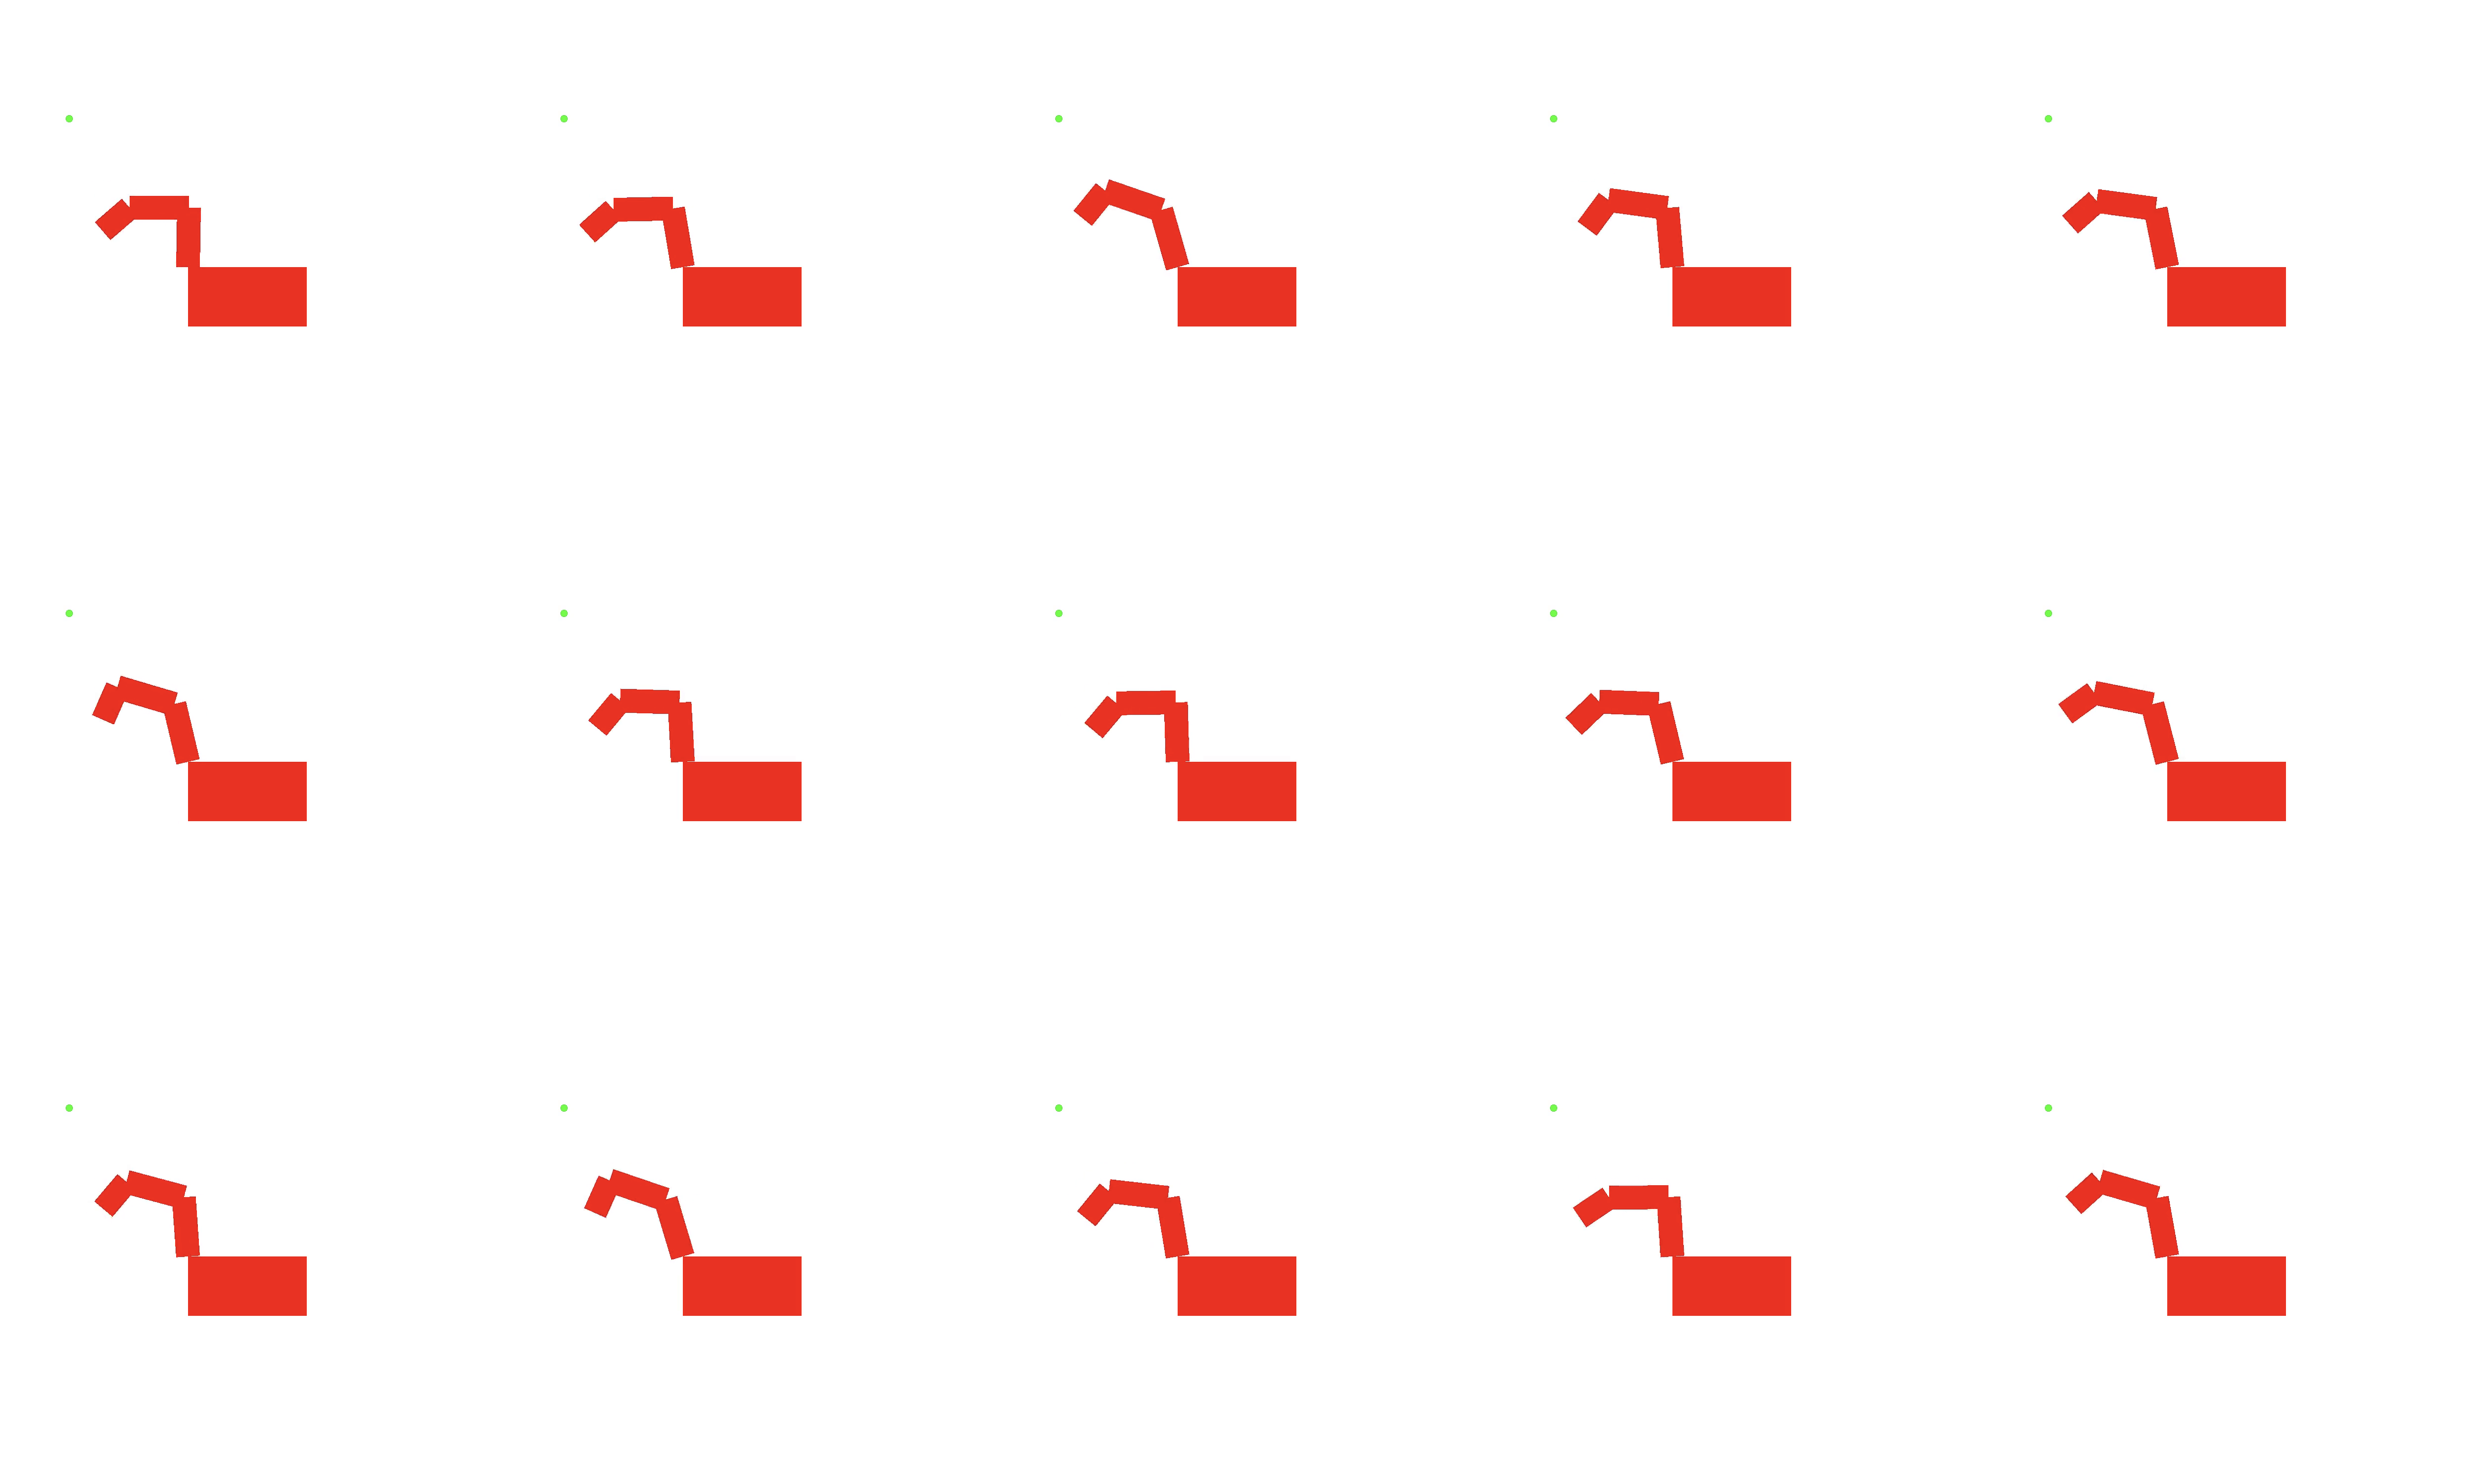
\includegraphics[width=1\textwidth]{figures/frames/frames_004.png}
      \caption{Control of a pigeon model with a static body trained on $r_{fifty\_fifty}$}
      \label{fig:fifty_fifty_body_speed_0}
  \end{figure}

  \begin{figure}[H]
      \centering
      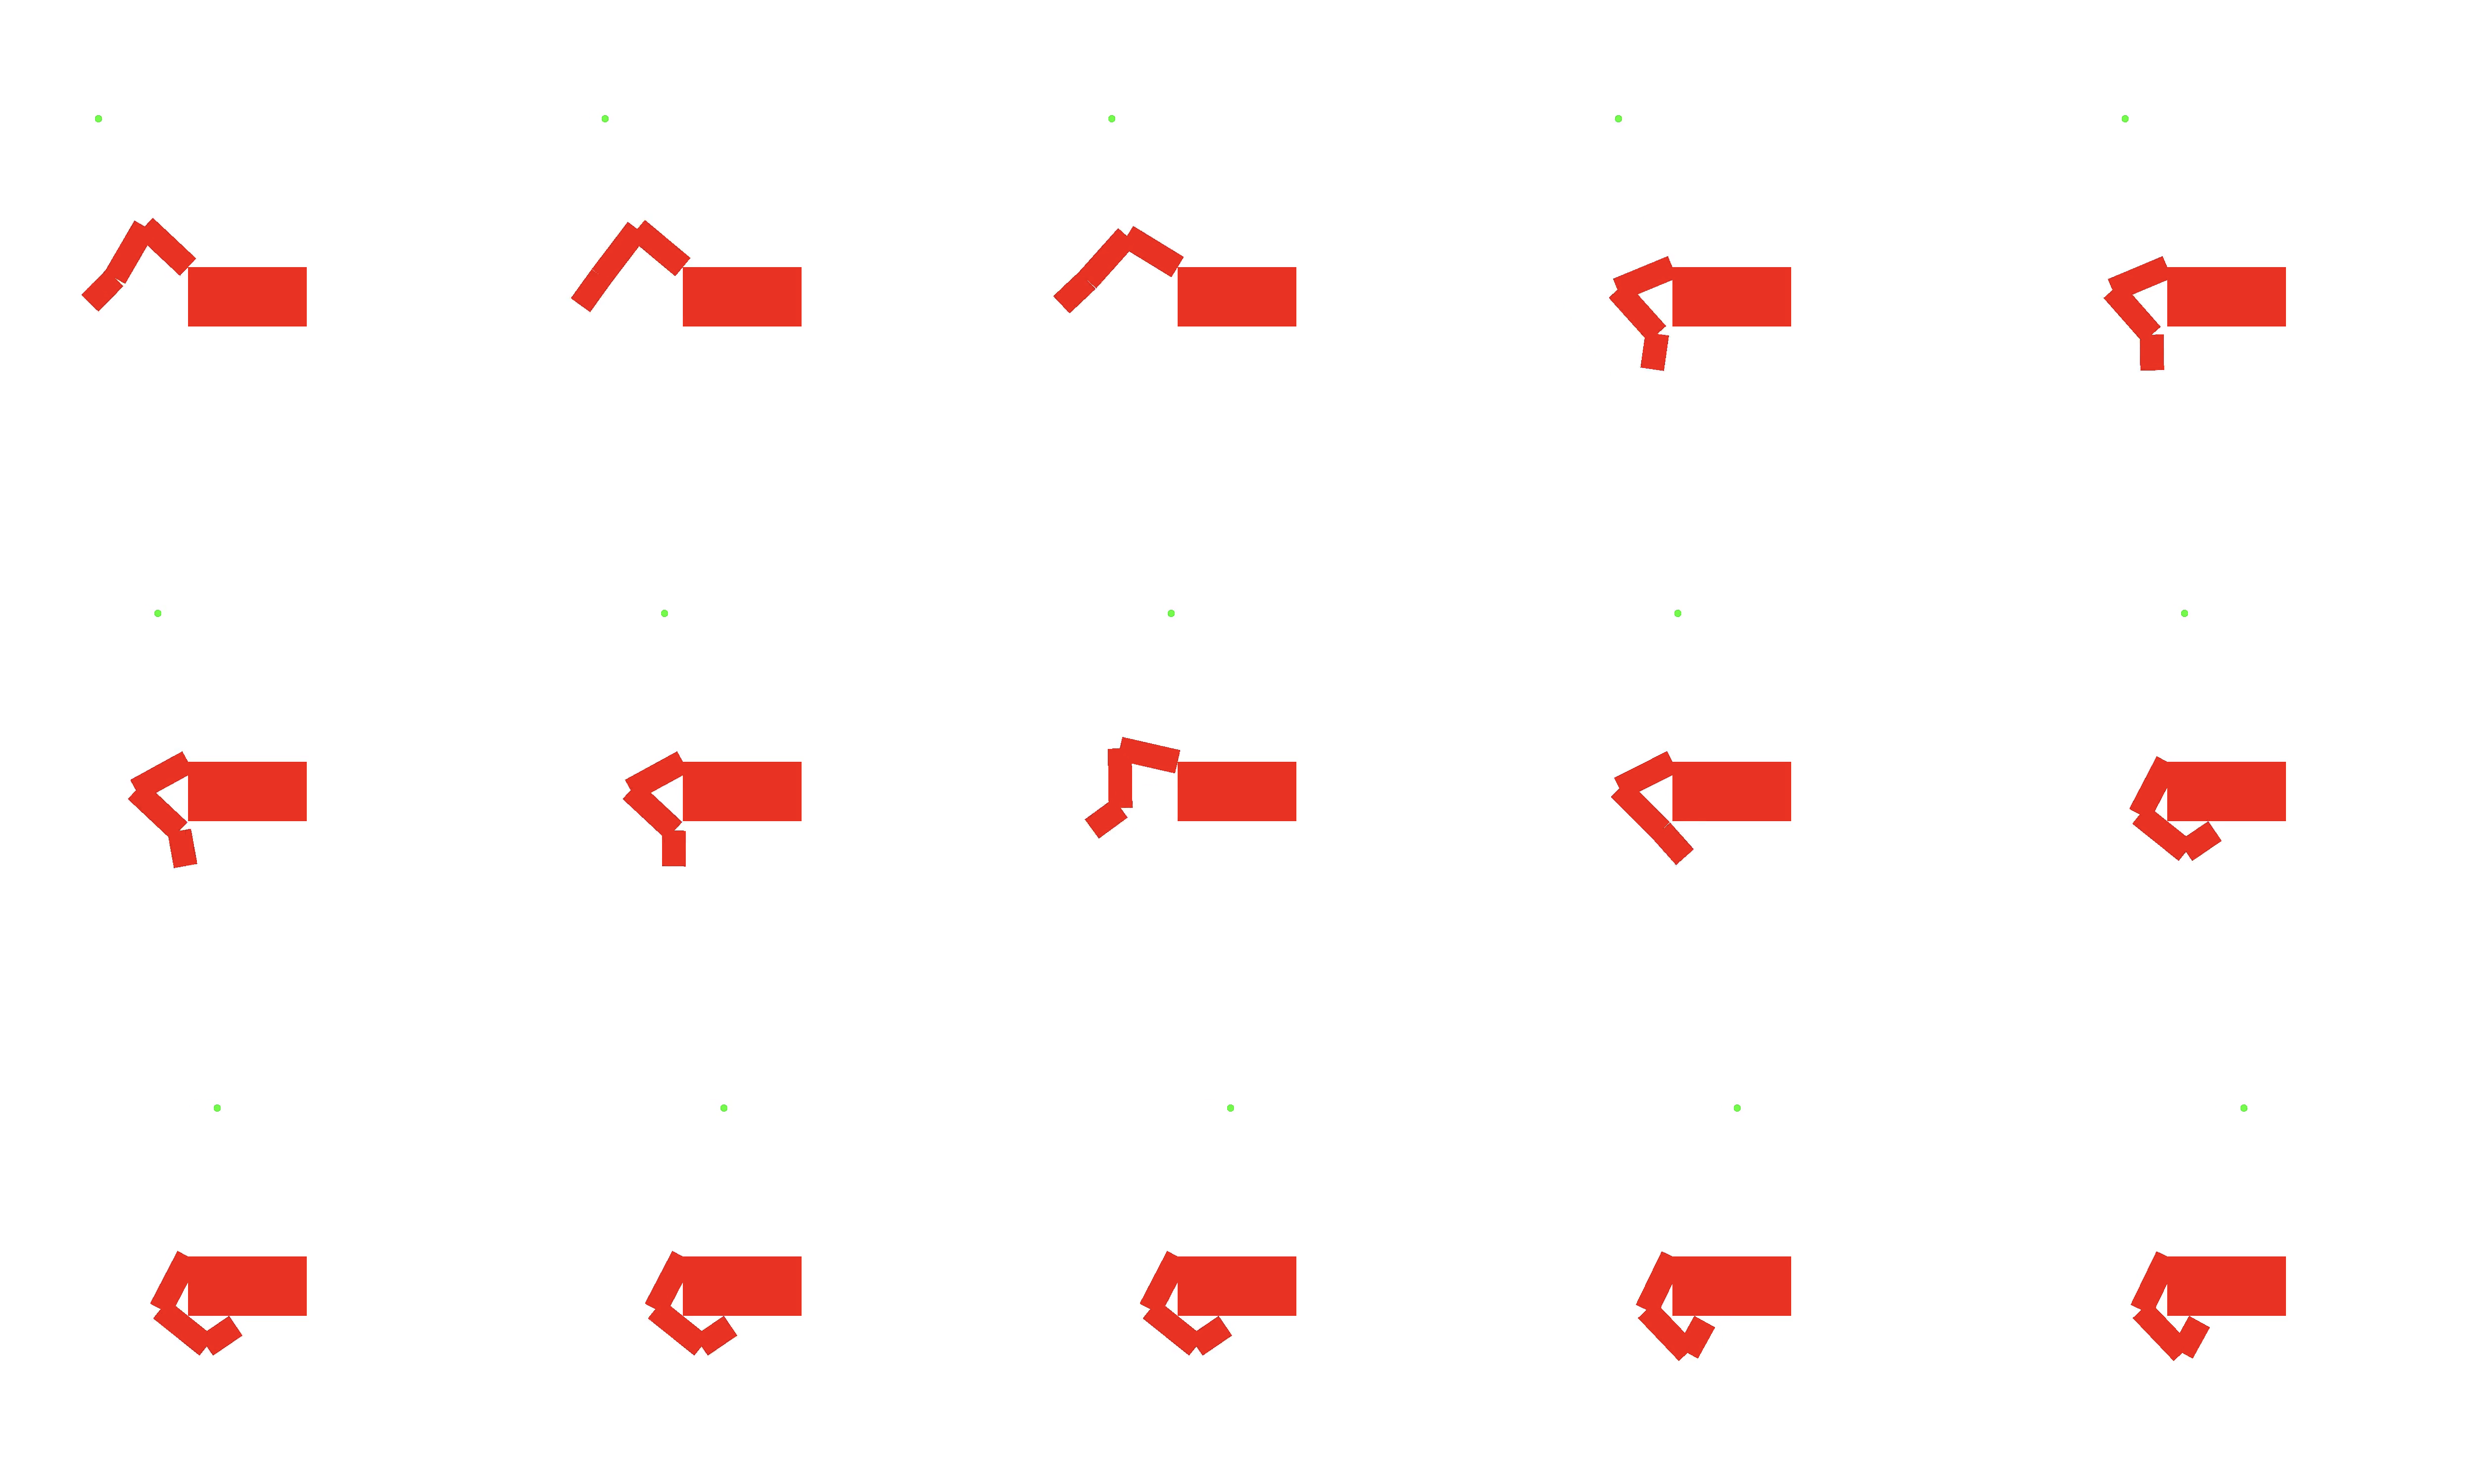
\includegraphics[width=1\textwidth]{figures/frames/frames_005.png}
      \caption{Control of a pigeon model with the body speed of 1 trained on $r_{fifty\_fifty}$}
      \label{fig:fifty_fifty_body_speed_1}
  \end{figure}


% summary of the results
